\documentclass{article}
\usepackage[utf8x]{inputenc}
\usepackage{ucs}
\usepackage{amsmath} 
\usepackage{amsfonts}
\usepackage{marvosym}
\usepackage{wasysym}
\usepackage{upgreek}
\usepackage[english,russian]{babel}
\usepackage{graphicx}
\usepackage{float}
\usepackage{textcomp}
\usepackage{hyperref}
\usepackage{geometry}
  \geometry{left=2cm}
  \geometry{right=1.5cm}
  \geometry{top=1cm}
  \geometry{bottom=1.8cm}
\usepackage{tikz}
\usepackage{ccaption}
\usepackage{multicol}
\hypersetup{
   colorlinks=true,
   citecolor=blue,
   linkcolor=black,
   urlcolor=blue
}
\usepackage{listings}
\usepackage[absolute]{textpos}
\usepackage{colortbl,graphicx,tikz}
\definecolor{X}{rgb}{.5,.5,.5}


\begin{document}
\pagenumbering{gobble}
\lstset{
  language=C,
  basicstyle=\linespread{1.1}\ttfamily,
  columns=fixed,
  fontadjust=true,
  basewidth=0.5em,
  keywordstyle=\color{blue}\bfseries,
  commentstyle=\color{gray},
  stringstyle=\ttfamily\color{orange!50!black},
  showstringspaces=false,
  numbersep=5pt,
  numberstyle=\tiny\color{black},
  numberfirstline=true,
  stepnumber=1,
  numbersep=10pt,
  backgroundcolor=\color{white},
  showstringspaces=false,
  captionpos=b,
  breaklines=true,
  breakatwhitespace=true,
  xleftmargin=.2in,
  extendedchars=\true,
  keepspaces = true,
  emph = {size_t},
  emphstyle={\color{blue}\bfseries},
}
\lstset{literate=%
   *{0}{{{\color{red!20!violet}0}}}1
    {1}{{{\color{red!20!violet}1}}}1
    {2}{{{\color{red!20!violet}2}}}1
    {3}{{{\color{red!20!violet}3}}}1
    {4}{{{\color{red!20!violet}4}}}1
    {5}{{{\color{red!20!violet}5}}}1
    {6}{{{\color{red!20!violet}6}}}1
    {7}{{{\color{red!20!violet}7}}}1
    {8}{{{\color{red!20!violet}8}}}1
    {9}{{{\color{red!20!violet}9}}}1
}
\newpage
\newgeometry{left=2cm,right=2cm,top=1cm,bottom=1.5cm}

\title{Семинар \#6: Динамический массив.\vspace{-5ex}}\date{}\maketitle

\section*{Разные варианты массивов в языке C}
\subsection*{Статический массив}
\begin{raggedleft}
\textit{Статический массив} -- это массив, размер которого фиксирован. В языке C такой массив создается так:
\end{raggedleft}
\begin{lstlisting}
int a[3] = {10, 20, 30};  
\end{lstlisting}
У такого статического массива есть 2 проблемы:
\begin{itemize}
\item Нельзя поменять размер, то есть нельзя добавить или удалить элемент.
\item Он выделяется на стеке и его максимальный размер сильно ограничен.
\end{itemize}


\subsection*{Массив на стеке с переменным размером, но фиксированной вместимостью}
Первую проблему можно частично решить, если создать массив больше, чем нужно на данный момент:
\begin{lstlisting}
int a[100] = {10, 20, 30};
size_t size = 3;
\end{lstlisting}
В этом примере мы создали статический массив, который может хранить 100 элементов, но в данный момент используем только первые 3 элемента. Чтобы помнить, сколько элементов используется в данный момент мы завели переменную \texttt{size}. Введём следующие определения:
\begin{itemize}
\item \textit{Размер массива (англ. size)} -- количество элементов массива, которые доступны для использования.
\item \textit{Вместимость массива (англ. capacity)} -- количество элементов, под которые в массиве выделена память.
\end{itemize}
То есть, для массива из примера выше размер равен 3, а вместимость равна 100.
В такой массив мы можем добавлять элементы, но только до тех пор пока размер меньше, чем вместимость. Например, добавить новый элемент в конец массива \texttt{a} можно так (но только если \texttt{size < 100}):
\begin{lstlisting}
a[size] = 60;
size += 1;
\end{lstlisting}
Несмотря на то, что в такой массив можно добавлять и удалять элементы, у такого подхода также есть недостатки. Вместимость не может меняться во время выполнения программы. Её нужно указать заранее. Если указать слишком маленькую вместимость, то этого может не хватить, а если указать слишком большую, то будет напрасно потрачено слишком много памяти. К тому же этот массив всё так же создаётся на стеке, поэтому его размер ограничен.

\subsection*{Выделение динамического массива в куче}
\textit{Динамический массив} -- это массив, размер и вместимость которого может меняться во время выполнения программы. Такой массив, можно создать, выделив память в куче:
\begin{lstlisting}
int* p = (int*)malloc(sizeof(int) * 3);
\end{lstlisting}
Указатель \texttt{p} указывает на массив из пяти элементов, созданный в куче.
После того, как такой массив был создан, можно изменить его размер. Для этого нужно сделать следующее:
\begin{enumerate}
\item Выделить в куче ещё один участок памяти под новый массив большего размера.
\item Скопировать данные из старого массива в новый.
\item Освободить память старого массива.
\end{enumerate}




\subsubsection*{Процесс увеличения размера массива, созданного в куче}
Пусть изначально у нас есть массив из трёх элементов, созданный в куче.
Попытаемся добавить ещё один элемент в такой массив.


\noindent\begin{minipage}{.45\textwidth}
\begin{lstlisting}
1) Исходное положение

int* p = (int*)malloc(sizeof(int)*3);
p[0] = 10;
p[1] = 20;
p[3] = 30;
\end{lstlisting}
\end{minipage}
\begin{minipage}{.45\textwidth}
\includegraphics[scale=0.75]{../images/malloc_realocation1.png}
\end{minipage}
\quad\\
\quad\\
\quad\\


\noindent\begin{minipage}{.45\textwidth}
\begin{lstlisting}
2) Выделяем новый массив большей памяти

int* q = (int*)malloc(sizeof(int)*4);
\end{lstlisting}
\end{minipage}
\begin{minipage}{.45\textwidth}
\includegraphics[scale=0.75]{../images/malloc_realocation2.png}
\end{minipage}
\quad\\
\quad\\
\quad\\


\noindent\begin{minipage}{.45\textwidth}
\begin{lstlisting}
3) Копируем элементы из старого массива
   и добавляем новый элемент
   
for (size_t i = 0; i < 3; ++i)
    q[i] = p[i];
q[3] = 40;
\end{lstlisting}
\end{minipage}
\begin{minipage}{.45\textwidth}
\includegraphics[scale=0.75]{../images/malloc_realocation3.png}
\end{minipage}
\quad\\
\quad\\
\quad\\


\noindent\begin{minipage}{.45\textwidth}
\begin{lstlisting}
4) Освобождаем память старого массива

free(p);
\end{lstlisting}
\end{minipage}
\begin{minipage}{.45\textwidth}
\includegraphics[scale=0.75]{../images/malloc_realocation4.png}
\end{minipage}
\quad\\
\quad\\
\quad\\


\noindent\begin{minipage}{.45\textwidth}
\begin{lstlisting}
5) Изменяем значение старого указателя

p = q;
\end{lstlisting}
\end{minipage}
\begin{minipage}{.45\textwidth}
\includegraphics[scale=0.75]{../images/malloc_realocation5.png}
\end{minipage}
\quad\\
\quad\\
\quad\\

Такой подход позволяет создавать массивы с изменяемым размером, не ограниченным размером стека.
Однако, и этого подхода есть недостатки:
\begin{itemize}
\item Медленное добавление элементов. Для того, чтобы добавить один элемент в массив, нам пришлось вызвать \texttt{malloc}, так же скопировать весь массив.
\item Придётся делать все операции по выделению/освобождению памяти и копированию массива каждый раз, когда нужно изменить размер. Это неудобно.
\end{itemize}



\newpage
\section*{Создаём свой динамический массив}

В отличии от многих других языков, в языке C нет удобного динамического массива, поэтому нам придётся написать свой. Попробуем написать наш массив так, чтобы он удовлетворял следующим требованиям:

\begin{enumerate}
\item В массив должно быть возможным добавление и удаление элементов. Его размер может меняться во время выполнения программы.
\item Размер массива не должен быть ограничен размером стека.
\item Массив должен быстро работать. Добавление и удаление элементов в конец массива должно работать за $O(1)$ в среднем. 
\item Массив не должен занимать слишком много памяти. А именно, общее количество выделенной для массива памяти должно быть не более чем в 2 раза превышать суммарный размер всех элементов массива.
\item С нашим массивом должно быть удобно работать.
\item Тип хранимого элемента массива должен быть настраиваемым.
\end{enumerate}
Структура для динамического массива будет выглядить следующим образом:
\begin{lstlisting}
struct dynarray 
{
    int* data;
    size_t size;
    size_t capacity;
};
typedef struct dynarray Dynarray;
\end{lstlisting}
Поля этой структуры:
\begin{itemize}
\item \texttt{data} -- указатель на элементы массива, которые выделяются в куче.
\item \texttt{size} -- текущий размер массива. Столько элементов содержится в массиве.
\item \texttt{capacity} - текущая вместимость массива. Под столько элементов в массиве выделена память. В отличии от статического массива эта величина может меняться. Количество памяти, выделенной в куче, будет равна \texttt{capacity * sizeof(int)}.
\end{itemize}
В памяти динамический массив с размером 5 и вместимостью 8 будет выглядеть следующим образом:
\begin{center}
\includegraphics[scale=1]{../images/dynarray1.png}
\end{center}



\newpage
\subsection*{Задачи:} 
Напишите следующие функции для работы с динамическим массивом:
\begin{itemize}
\item \texttt{Dynarray dynarray\_create(size\_t initial\_capacity)} -- эта функция должна создавать динамический массив с размером равным нулю и вместимостью равной \texttt{initial\_capacity}. Память должна выделяться в куче с помощью \texttt{malloc}.

\item \texttt{void dynarray\_destroy(Dynarray* d)} -- эта функция должна освобождать выделенную память (\texttt{free}).

\item Перепишите все функции из прошлой части: \texttt{dynarray\_push\_back}, \texttt{dynarray\_print} и другие.

\item \textbf{Расширение массива:} Измените код так, чтобы происходило перевыделение памяти тогда, когда размер массива начинает превышать вместимость в функциях \texttt{dynarray\_push\_back} и \texttt{dynarray\_insert}. Вместимость динамического массива должна увеличиваться в 2 раза.  Это можно сделать двумя способами:
\begin{itemize}
\item Выделить новый участок памяти в 2 раза больше прежнего, используя \texttt{malloc}. Переписать все элементы в новую память. Освободить старую память с помощью \texttt{free}.
\item Использовать функцию \texttt{realloc}, которая будет делать то же самое, но более эффективно.
\end{itemize}

\item \textbf{Проверка на корректность:} Функции \texttt{malloc} и \texttt{realloc} не всегда могут выделить необходимую память. Например, если вы запросите больше чем вся оперативная память, то они ничего не смогут сделать. В этом случае эти функции возвращают нулевой указатель (т.е. указатель, равный \texttt{NULL}). В случае возникновения такой ошибки \texttt{realloc} не освобождает старую память. Добавьте в программу проверки на возникновения таких ошибок. Если память выделить нельзя, то программа должна печатать сообщение о нехватке памяти и завершаться.

\item \textbf{Размер и вместимость:}
Напишите программу, которая будет создавать стек вместимости \texttt{1} и добавлять в него последовательно \texttt{200} элементов. При каждом добавлении элемента печатайте размер и вместимость.\\

\item \textbf{Другие типы элементов:} Предположим, что вы однажды захотите использовать динамический массив не для целочисленных чисел типа \texttt{int}, а для какого-нибудь другого типа (например \texttt{char}). Введите синоним для типа элементов динамического массива:
\begin{verbatim}
typedef int Data;
\end{verbatim}
Измените тип элемента динамического массива во всех функциях с \texttt{int} на \texttt{Data}. Теперь вы в любой момент сможете изменить тип элементов стека, изменив лишь одну строчку.
\end{itemize}


\newpage
\section*{Заголовочные файлы}


\newpage
\section*{Абстрактные типы данных: Стек и Очередь}
\textbf{Абстракстный тип данных (АТД)} - это математическая модель для типов данных, которая задаёт поведение этих типов, но не их внутреннею реализацию.\\

\textbf{Стек (Stack, не путайте с сегментом памяти под таким же названием!)} - это АТД, который представляет собой коллекцию элементов, менять которые можно только с помощью двух операций:
\begin{itemize}
\item \texttt{push} - добавить элемент в стек.
\item \texttt{pop} - извлечь из стека последний добавленный элемент.
\end{itemize}
Таким образом, поведение стека задаётся этими двумя операциями. Так как стек - это абстрактный тип данных, то его внутренняя реализация на языке программирования может быть самой разной. Стек можно сделать на основе статического массива, на основе динамического массива или на основе связного списка. Внутренняя реализация не важна, важно только наличие операций \texttt{push} и \texttt{pop}. \\
Не нужно путать абстракстный тип данных стек с сегментом памяти стек.\\

\textbf{Очередь (Queue)} - это АТД, который представляет собой коллекцию элементов, менять которые можно только с помощью двух операций:
\begin{itemize}
\item \texttt{enqueue} - добавить элемент в очередь.
\item \texttt{dequeue} - извлечь из очереди первый добавленный элемент из оставшихся.
\end{itemize}

\begin{center}
\includegraphics[scale=0.31]{../images/stack_queue.png}
\end{center}

\textbf{Дек (Deque = Double-ended queue)} - это АТД, который представляет собой коллекцию элементов, менять которые можно только с помощью четырёх операций:
\begin{itemize}
\item \texttt{push\_back} - добавить элемент в конец.
\item \texttt{push\_front} - добавить элемент в начало.
\item \texttt{pop\_back} - извлечь элемент с конца.
\item \texttt{pop\_front} - извлечь элемент с начала.\\
\end{itemize}

\textbf{Очередь с приоритетом (Priority Queue)} - это АТД, который представляет собой коллекцию элементов, менять которые можно только с помощью двух операций:
\begin{itemize}
\item \texttt{insert} - добавить элемент.
\item \texttt{extract\_best} - извлечь из очереди элемент с наибольшим приоритетом. 
\end{itemize}
То, что будет являться приоритетом может различаться. Это может быть как сам элемент, часть элемента (например, одно из полей структуры) или другие данные, подаваемые на вход операции \texttt{insert} вместе с элементом. В простейшем случае, приоритетом является сам элемент (тогда очередь с приоритетом просто возвращает максимальный элемент) или сам элемент со знаком минус (тогда очередь с приоритетом возвращает минимальный элемент).


\newpage
\section*{Реализация стека на основе динамического массива}

\begin{center}
\includegraphics[width=0.6\linewidth]{../images/stack.png}
\end{center}

\subsection*{Задачи:}
\begin{itemize}
\item Напишите следующие функции:
\begin{enumerate}
\item \texttt{void stack\_push(Stack* s, Data x)} -- добавляет элемент в стек.
\item \texttt{Data stack\_get(const Stack* s)} -- возвращает элемент, находящийся в вершине стека, но не изменяет стек.
\item \texttt{void stack\_pop(Stack* s)} -- удаляет элемент, находящийся в вершине стека. 
\item \texttt{int stack\_is\_empty(const Stack* s)} -- возвращает 1 если стек пуст и 0 иначе.
\item \texttt{void stack\_print(const Stack* s)} -- распечатывает все элементы стека.
\end{enumerate}



\item \textbf{Скобочки}: Написать программу которая будет считывать последовательность скобочек и
печатать \texttt{Yes} или \texttt{No} в зависимости от того является ли эта последовательность допустимой. Для считывания строки: \texttt{scanf(``\%s'', str);}
\begin{multicols}{2}
\begin{center}
\begin{tabular}{ c | c }
 вход & выход \\ \hline
 \texttt{()} & Yes \\
 \texttt{\{[()]\}} & Yes  \\ 
 \texttt{)))))}  &  No \\ 
 \texttt{([)]}  &  No \\ 
 \texttt{[\{\}()]}  &  Yes \\ 
\end{tabular}
\end{center}

\begin{center}
\begin{tabular}{ c | c }
 вход & выход \\ \hline
 \texttt{)(}  &  No \\
 \texttt{((((((()))))))} & Yes \\
 \texttt{\{\{\{\{} & No  \\ 
 \texttt{\{[([]()[\{\}])][()]\}}  &  Yes \\ 
 \texttt{]}  &  No \\ 
\end{tabular}
\end{center}
\end{multicols}


\item \textbf{Следующий больший}: На вход поступает последовательность чисел. Нужно найти, для каждого элемента, индекс первого элемента, который следует после данного и является больше данного. Если такого элемента нет, то нужно напечатать \texttt{-1}.
\begin{center}
\begin{tabular}{ l | l }
 вход & выход \\ \hline
 \texttt{10} &  \texttt{1 4 3 4 5 -1 7 -1 -1 -1}\\
 \texttt{1 5 2 4 6 9 1 8 7 3} & \\ \hline
 
 \texttt{5} &  \texttt{1 2 3 4 -1}\\
 \texttt{1 2 3 4 5} & \\ \hline
 
  \texttt{2} &  \texttt{-1 -1}\\
 \texttt{2 1} & \\
\end{tabular}
\end{center}

\end{itemize}













\iffalse
\section*{Массив фиксированного размера внутри структуры}
В файле \texttt{0array\_in\_struct.c} содержится минимальный пример массива, который хранится внутри структуры. Максимальная вместимость массива равна \texttt{100}. А размер хранится внутри структуры и может принимать значения от 0 до 100. Функция \texttt{push\_back} принимает на вход адрес на такую структуру и число \texttt{value}, а затем добавляет это число в конец массива.\\

Зачем хранить массив внутри структуры, если можно было бы просто создать его без струтуры? На самом деле у такого подхода много преимуществ:
\begin{enumerate}
\item Он позволяет нам самим описать поведение массива при добавлении и удалении элементов.
\item Мы можем передавать такой массив внутри функций также как и обычные переменные.
\item Такой подход распространяется на более сложные структуры данных
\end{enumerate}

\subsection*{Задачи:} 
Напишите следующие функции для работы с этим массивом:
\begin{itemize}
\item \texttt{array\_print} -- эта функция должна принимать на вход адрес структуры \texttt{Array} и печатать массив на экран.
\item \texttt{array\_is\_empty} -- эта функция должна принимать на вход адрес структуры \texttt{Array} и возвращать \texttt{1}, если массив пуст и \texttt{0} иначе.
\item \texttt{int array\_get(const Array* a, int index)} эта функция должна возвращать число, которое лежит по индексу \texttt{index} в массиве.
\item \texttt{void array\_set(const Array* a, int index, int value)} -- эта функция должна устанавливать элемент массива, лежащий по индексу \texttt{index} значением \texttt{value}.
\item \texttt{void array\_erase(const Array* a, int index)} -- эта функция должна удалять элемент под индексом \texttt{index}. При этом, конечно, все элементы, которые следовали после удаляемого нужно сместить влево на 1 элемент.
\item \texttt{void array\_insert(const Array* a, int index)} -- эта функция должна вставлять элемент в массив в место между элементами с индексами \texttt{index - 1} и \texttt{index}. При этом, конечно, все элементы, которые находились правее этого места, должны сместиться вправо на один элемент.
\item \texttt{void array\_append(Array* a, const Array* b)} -- эта функция должна добавлять всё содердимое массива \texttt{b} в конец массива \texttt{a}.

\item \textbf{Проверка индекса:} Как известно, в языке \texttt{C} у статических массивов нет проверки на выход за пределы массива. Например, следующий код может сработать и не выдасть никакой ошибки.
\begin{lstlisting}
int array[100] = {};
printf("%i\n", array[101]);
\end{lstlisting}
Компилятор просто преобразует строку \texttt{array[101]} в \texttt{*(array + 101)} и обратится к соответствующему участку памяти.
Причина того, что в \texttt{C} нет такой проверки заключается в том, что она бы немного замедлила программу. Язык \texttt{C} ориентирован на максимальное быстродействие, поэтому и не делает такую проверку. 

Однако, за отсутствие такой проверки приходится платить тем что в программе могут появиться сложно выявляемые ошибки. Например, если вы случайно ошибётесь с индексами массива, то можете этого даже не заметить. Программа будет работать с памятью за пределами этого массива и почти всегда выдавать правильные результаты. Но иногда, выходя за пределы массива вы можете изменить другие переменные. Найти такую ошибку в большой программе может быть очень сложно.

Добавьте в нашу реализацию массива проверку на принадлежность индекса правильному диапазону значений в функции \texttt{array\_get} и \texttt{array\_set}. Если индекс не входит в правильный диапазон, программа должна печатать сообщение об ошибке и завершаться. Завершить программу можно с помощью вызова \texttt{exit(1)}, функции \texttt{exit} из библиотеки \texttt{stdlib.h}. 

\item \textbf{Вместимость:} Текущая вместимость нашего массива -- всего 100 элементов. Если размер массива превысит это значение, то тоже должна происходить ошибка. Добавьте проверку на превышение вместимости в функции \texttt{array\_insert} и \texttt{array\_append}. Чтобы не писать везде магическое число \texttt{100}, введите константу, которая будет задавать вместимость.
\end{itemize}
\fi


\end{document}